\documentclass[11pt,letterpaper]{article}

\usepackage[
  letterpaper,
  left=0.6in,
  right=0.6in,
  top=0.8in,
  bottom=0.8in,
  headheight=14pt,
  headsep=0.25in,
  footskip=0.35in
]{geometry}

\usepackage{fontspec}
\setmainfont{Google Sans}
\usepackage{microtype}

\usepackage{amsmath}
\usepackage{amssymb}
\usepackage{booktabs}
\usepackage{array}
\usepackage{multirow}
\usepackage{tabularx}
\usepackage{graphicx}
\usepackage{caption}
\usepackage{enumitem}
\usepackage[section]{placeins}
\usepackage[hidelinks]{hyperref}
\usepackage{tikz}
\usetikzlibrary{fit,positioning,calc,arrows.meta}
\usepackage{xcolor}
\usepackage{float}
\usepackage{needspace}
\renewcommand{\topfraction}{0.9}
\renewcommand{\floatpagefraction}{0.8}

\graphicspath{{figures/}}
\captionsetup{font=small,labelfont=bf,labelsep=period,skip=6pt}
\setlist[itemize]{leftmargin=1.2em,itemsep=2pt,topsep=3pt,parsep=0pt}
\setlist[enumerate]{leftmargin=1.4em,itemsep=2pt,topsep=3pt,parsep=0pt}
\setlength{\parskip}{4pt}
\setlength{\emergencystretch}{2em}

\pagestyle{plain}

\setlength{\parindent}{0pt}

\newcommand{\todo}[1]{\textcolor{red}{\textbf{[#1]}}}
\newcommand{\taskbanner}[2]{\begin{center}{\small\bfseries #1}\\[3pt]{\Large\bfseries #2}\end{center}\vspace{2pt}\hrule\vspace{8pt}}

\begin{document}

\begin{center}
  {\small\bfseries AI651: Deep Learning for Space, Time and Graphs}\\[6pt]
  {\Large\bfseries Assignment 2}\\[6pt]
  {\small Question 1: River Forecasting Proposal; Question 2: Motion or Memory?}
\end{center}

\vspace{2pt}
\noindent\begin{tabular}{@{}p{0.8in}p{5.6in}@{}}
\textbf{Name}      & Muhammad Hussain Habib \\
\textbf{Roll no.}  & 27100016 \\
\textbf{Repository} & \texttt{https://github.com/Hussain004/DL4STG-PA2} \\
\end{tabular}

\vspace{6pt}
\normalsize

\taskbanner{Question 1}{River Forecasting Proposal}

My proposal is a small model with a lot of structure in it. There is one grid
that holds every source, a temporal encoder that runs on each place separately,
and four rounds of message passing along the directed river graph. Every edge of
the graph has a learned lag kernel, so the model estimates the transport time
itself instead of me guessing it. The reasoning comes from the first experiment
in the companion notebook, where a model that cannot see its neighbour cannot
use what the neighbour knows. A river forecaster has the same problem, and giving
it the graph is the same fix.

There is no data for this catchment, so the
design is argued from what the question tells us: the four hops between the dam
and S4, the travel times quoted in the tutorial, the fact that travel times
change with river conditions, and the experiments in the companion notebook. In
Section 4.6 I run one small sanity check on a synthetic river that I generated
with Claude Code (the prompt is in the declaration at the end). Those numbers
only show that the design trains and behaves the way I expect. They say nothing
about the real river, and I do not use them anywhere else.

\section*{1. Architecture diagram}

The whole system is one tensor. I stack every place and every channel on a common
10-minute grid, so the model never has to align the sources by itself:

\begin{center}
\begin{tabular}{@{}p{0.95in}p{5.5in}@{}}
\textbf{Grid}      & a $30\times6\times4$ grid, B $\times$ 30 $\times$ 6 $\times$ 4 for a batch \\
\textbf{Places}   & Dam, S1, T1, S2, S3, S4 (6 rows) \\
\textbf{Time}     & 24 observed steps $+$ 6 forecast steps (30 columns) \\
\textbf{Channels} & $[$level, observed?, rain, release$]$ (4 channels) \\
\textbf{Forecast} & 4 stations $\times$ 6 steps, B $\times$ 4 $\times$ 6 levels in metres \\
\end{tabular}
\end{center}

\begin{figure}[!t]
\centering
\resizebox{0.95\linewidth}{!}{%
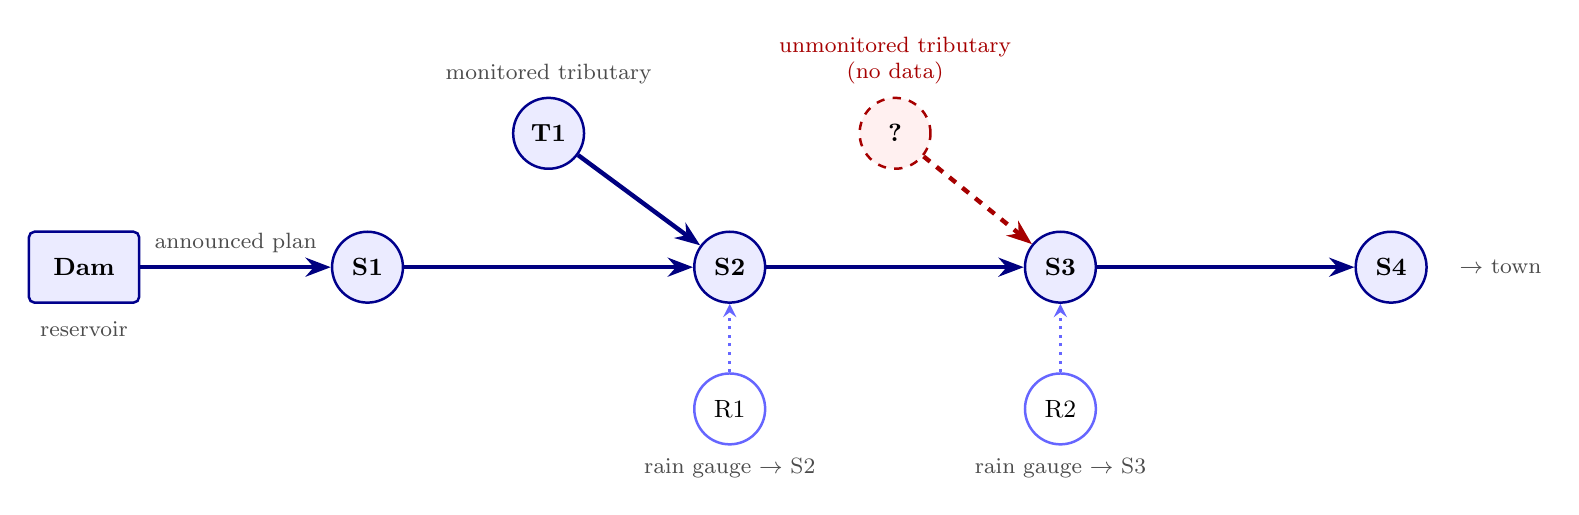
\begin{tikzpicture}[font=\small, >=stealth,
  st/.style={circle, draw=blue!55!black, fill=blue!8, line width=0.9pt, minimum size=9mm, inner sep=0pt, font=\small\bfseries},
  un/.style={circle, draw=red!65!black, fill=red!6, line width=0.9pt, minimum size=9mm, inner sep=0pt, dashed},
  gg/.style={circle, draw=blue!60, fill=white, line width=0.9pt, minimum size=9mm, inner sep=0pt},
  river/.style={line width=1.6pt, draw=blue!50!black, -{Stealth[length=3.2mm]}},
  note/.style={font=\footnotesize, text=black!70, align=center}]
\node[draw=blue!55!black, fill=blue!8, line width=0.9pt, rounded corners=2pt, minimum width=14mm, minimum height=9mm, font=\small\bfseries] (dam) at (0,0) {Dam};
\node[st] (s1) at (3.6,0) {S1};
\node[st] (s2) at (8.2,0) {S2};
\node[st] (s3) at (12.4,0) {S3};
\node[st] (s4) at (16.6,0) {S4};
\node[st] (t1) at (5.9,1.7) {T1};
\node[un] (u)  at (10.3,1.7) {\textbf{?}};
\node[gg] (r1) at (8.2,-1.8) {R1};
\node[gg] (r2) at (12.4,-1.8) {R2};
\draw[river] (dam) -- node[above=1pt, note]{announced plan} (s1);
\draw[river] (s1) -- (s2);
\draw[river] (s2) -- (s3);
\draw[river] (s3) -- (s4);
\draw[river] (t1) -- (s2);
\draw[river, draw=red!65!black, dashed] (u) -- (s3);
\draw[->, dotted, line width=1.1pt, draw=blue!60] (r1) -- (s2);
\draw[->, dotted, line width=1.1pt, draw=blue!60] (r2) -- (s3);
\node[note, above=1pt of t1] {monitored tributary};
\node[note, text=red!65!black, above=1pt of u] {unmonitored tributary\\(no data)};
\node[note, below=1pt of r1] {rain gauge $\to$ S2};
\node[note, below=1pt of r2] {rain gauge $\to$ S3};
\node[note, below=3pt of dam] {reservoir};
\node[note, right=8pt of s4] {$\to$ town};
\end{tikzpicture}}\\[6pt]
\begin{minipage}[t]{0.52\linewidth}
\centering
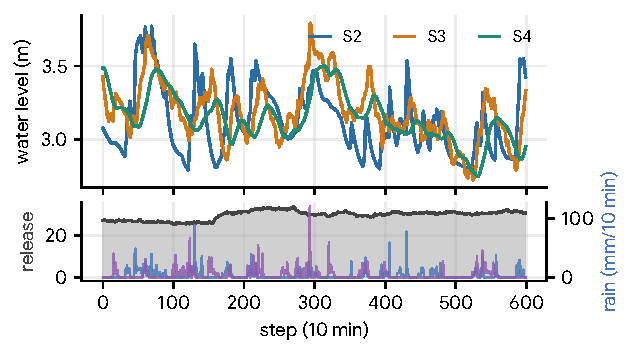
\includegraphics[width=\linewidth]{fig_river_series.pdf}
\end{minipage}\hfill
\begin{minipage}[t]{0.44\linewidth}
\centering
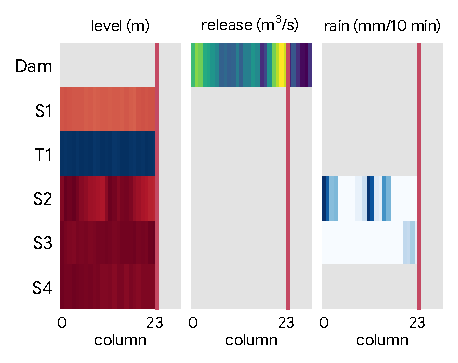
\includegraphics[width=\linewidth]{fig_river_grid.pdf}
\end{minipage}
\caption{The catchment and the grid. \textbf{Top:} the river as a directed graph.
Solid arrows are flow; T1 joins between S1 and S2, the unmonitored tributary
(dashed, no data) joins between S2 and S3, and the rain gauges (dotted) are folded
into S2 and S3. \textbf{Bottom left:} a stretch of the synthetic river used for the
sanity check, where a change in the Dam release reaches the stations later.
\textbf{Bottom right:} the grid the model sees (24 observed and 6 forecast columns).
Grey cells hold no data. The red line is the forecast origin; to its right the only
non-empty content is the announced release plan in the Dam row.}
\label{fig:river}
\end{figure}

\subsection*{1.1 The sources and how they are combined}

\begin{itemize}
\item \textbf{Levels at S1--S4 and T1.} One value every 10 minutes, with noise,
some missing readings and some late ones. Each goes into the level channel of its
own row, and a second channel marks whether the reading exists.
\item \textbf{Rain at R1 and R2.} I bin these into 10-minute totals and put them
in the row of the place they drain into: R1 in the S2 row and R2 in the S3 row
(assumption A4).
\item \textbf{Reservoir.} Recorded releases go in the release channel of the Dam
row for the observed columns. The announced schedule for the coming hour goes in
the same channel for the six forecast columns.
\end{itemize}

Nothing else goes in. In particular, no future level and no future rainfall
reaches the model, because the forecast columns are empty and flagged as not
seen, except for the announced plan. The rule is simple: if I would not know it
at issuance time, the model cannot use it.

\subsection*{1.2 The three blocks}

\begin{figure}[htbp]
\centering
\resizebox{\linewidth}{!}{%
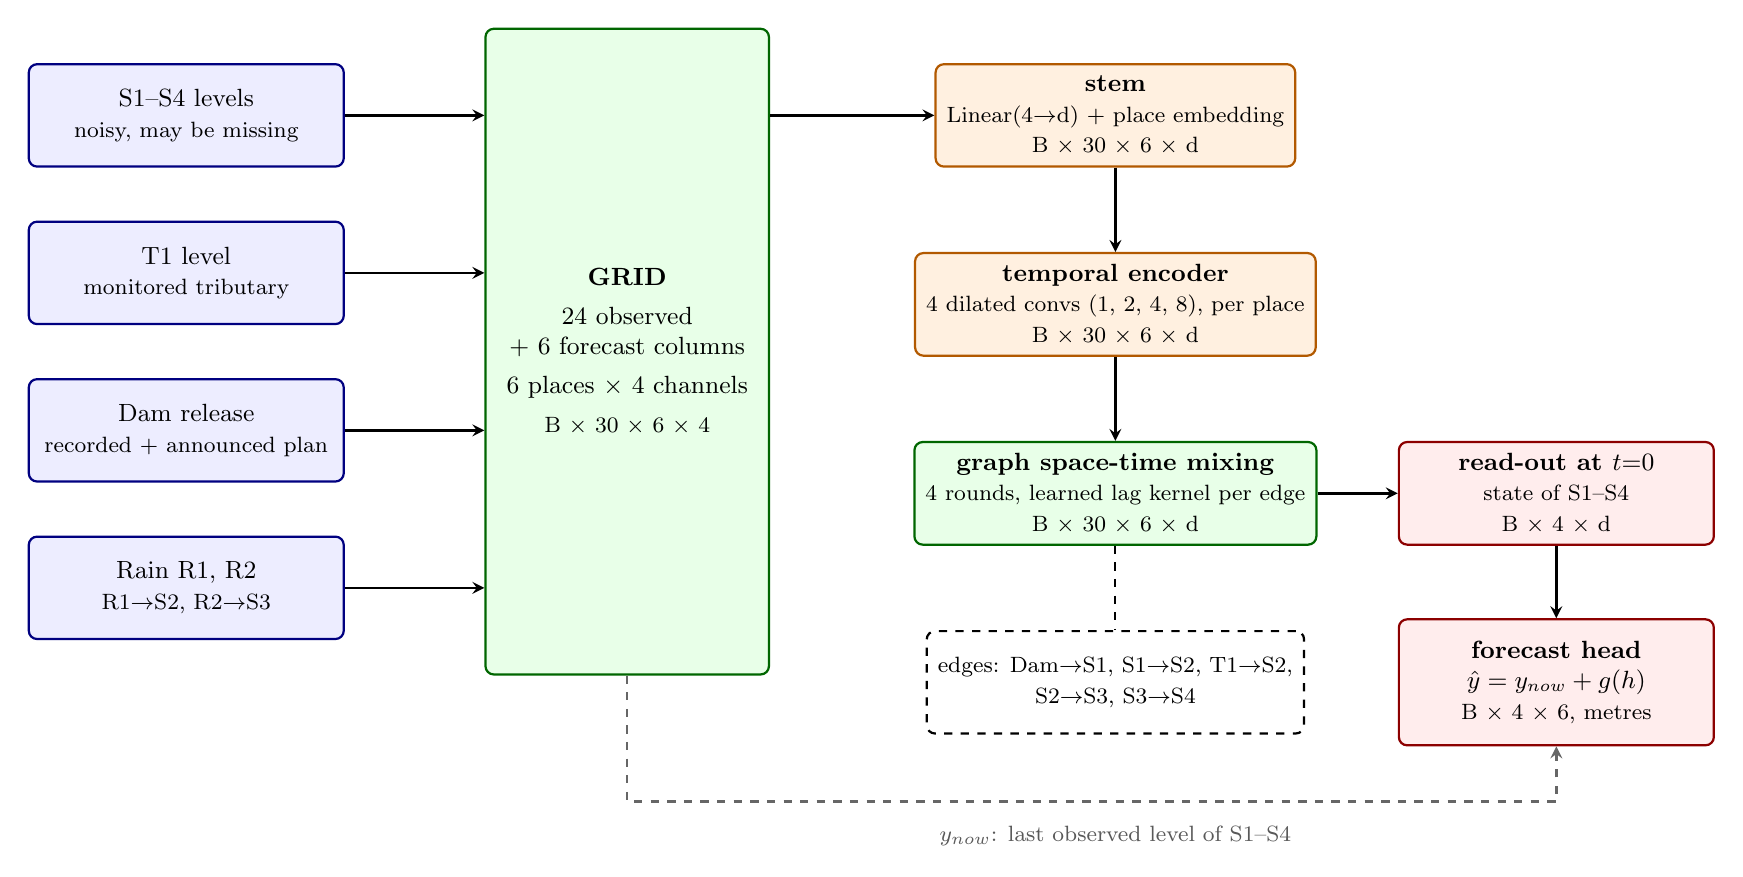
\begin{tikzpicture}[font=\small, >=stealth,
  box/.style={draw, rounded corners=3pt, align=center, inner sep=4pt, minimum height=13mm, line width=0.8pt},
  src/.style={box, fill=blue!7, draw=blue!50!black, minimum width=40mm},
  grd/.style={box, fill=green!9, draw=green!40!black, minimum width=36mm},
  enc/.style={box, fill=orange!12, draw=orange!70!black, minimum width=44mm},
  gph/.style={box, fill=green!9, draw=green!40!black, minimum width=44mm},
  outb/.style={box, fill=red!7, draw=red!55!black, minimum width=40mm},
  fl/.style={->, line width=0.9pt},
  tens/.style={font=\footnotesize, text=black!65}]
% sources
\node[src] (s1) at (0,8.4) {S1--S4 levels\\{\footnotesize noisy, may be missing}};
\node[src] (s2) at (0,6.4) {T1 level\\{\footnotesize monitored tributary}};
\node[src] (s3) at (0,4.4) {Dam release\\{\footnotesize recorded $+$ announced plan}};
\node[src] (s4) at (0,2.4) {Rain R1, R2\\{\footnotesize R1$\to$S2, R2$\to$S3}};
% grid: tall box so every source arrow is horizontal
\node[grd, minimum height=82mm] (grid) at (5.6,5.4) {\textbf{GRID}\\[3pt]24 observed\\$+$ 6 forecast columns\\[3pt]6 places $\times$ 4 channels\\[3pt]{\footnotesize B $\times$ 30 $\times$ 6 $\times$ 4}};
% pipeline
\node[enc] (stem) at (11.8,8.4) {\textbf{stem}\\{\footnotesize Linear(4$\to$d) $+$ place embedding}\\{\footnotesize B $\times$ 30 $\times$ 6 $\times$ d}};
\node[enc] (tcn)  at (11.8,6.0) {\textbf{temporal encoder}\\{\footnotesize 4 dilated convs (1, 2, 4, 8), per place}\\{\footnotesize B $\times$ 30 $\times$ 6 $\times$ d}};
\node[gph] (gmp)  at (11.8,3.6) {\textbf{graph space-time mixing}\\{\footnotesize 4 rounds, learned lag kernel per edge}\\{\footnotesize B $\times$ 30 $\times$ 6 $\times$ d}};
\node[box, fill=white, dashed, minimum width=44mm] (edges) at (11.8,1.2) {\footnotesize edges: Dam$\to$S1, S1$\to$S2, T1$\to$S2,\\\footnotesize S2$\to$S3, S3$\to$S4};
\node[outb] (ro)   at (17.4,3.6) {\textbf{read-out at $t{=}0$}\\{\footnotesize state of S1--S4}\\{\footnotesize B $\times$ 4 $\times$ d}};
\node[outb, minimum height=16mm] (head) at (17.4,1.2) {\textbf{forecast head}\\$\hat y = y_{now} + g(h)$\\{\footnotesize B $\times$ 4 $\times$ 6, metres}};
% flow
\foreach \i in {s1,s2,s3,s4} \draw[fl] (\i.east) -- (\i.east -| grid.west);
\draw[fl] (grid.east |- stem.west) -- (stem.west);
\draw[fl] (stem.south) -- (tcn.north);
\draw[fl] (tcn.south) -- (gmp.north);
\draw[fl] (gmp.east) -- (ro.west);
\draw[fl] (ro.south) -- (head.north);
\draw[dashed, line width=0.7pt] (gmp.south) -- (edges.north);
% residual skip: last observed level goes straight to the head
\draw[fl, dashed, draw=black!60] (grid.south) -- ++(0,-1.6) -| (head.south);
\node[tens, fill=white, inner sep=1pt] at (11.8,-0.75) {$y_{now}$: last observed level of S1--S4};
\end{tikzpicture}}
\caption{The three blocks. The grid is the only place where the sources meet. The
temporal encoder runs on each place separately with shared weights and a learned place
embedding, so the four stations share what they have in common while the dam can still
behave differently. The graph stage is the only place where one place can see another.}
\label{fig:blocks}
\end{figure}

\textbf{Alignment, projection and reshaping.} Three things change shape between
the grid and the output:

\begin{itemize}
\item \textbf{Alignment} happens once, when the grid is built. Rain is binned onto
the same 10-minute clock as the levels. The last observed level of each station is
carried forward through any gap and kept separately as $y^s_0$. The announced
schedule is written into the six forecast columns of the Dam row, one column per
future step.
\item \textbf{Projection} from 4 channels to $d{=}64$ features happens in the
stem. A learned place embedding of the same width is added, so the encoder can
treat the dam differently from a gauged station.
\item \textbf{Reshaping} happens twice inside the encoder. The grid is viewed as
$B\times6$ sequences of length 30 with 64 channels, convolved along time, and
folded back.
\end{itemize}

\subsection*{1.3 How far a forecast can reach}

A forecast can only use what has a path to it. The temporal encoder has a radius of $1+2+4+8=15$ steps around the read-out
index. Each round of message passing moves information one hop along the river,
and each edge can take its message from any lag in a window of 12 steps. So a
message can cross the four-hop path with a lag of up to 44 steps. This means the
S4 forecast can still be moved by the dam's release from 59 steps back, by S1
from 48, by S2 from 37, by S3 from 26 and by S4's own history from 15.

The dam is four hops from S4, which is why the graph mixing has four rounds. With
fewer rounds the dam's release could not reach S4 at all. The reach (59 steps) is
also much larger than the 24-step window I feed in, so the window is the limit
and not the network. If the authority tells me the real transit is longer than I
assume, I widen the window and nothing else changes.


\section*{2. Assumptions}

The question gives us some facts and leaves the rest open. The facts are:
10-minute sampling; four main stations plus a monitored tributary; two rain gauges
with stated locations; a reservoir with recorded releases and announced future
schedules, with announcement and effective times; and station locations, river
connectivity and distances along the river. It also says what is not supplied,
which is precise travel times and the inflow of the unmonitored tributary, and that
future rainfall and future water levels are not available at issuance.

Everything in the table below is my own assumption. For each one I give the reason
and what it changes in the design.

\begin{table}[H]
\centering
\small
\begin{tabularx}{\textwidth}{@{}p{0.2in}p{2.15in}p{2.15in}X@{}}
\toprule
\textbf{\#} & \textbf{I assume} & \textbf{because} & \textbf{therefore in my design} \\
\midrule
A1 & a station reports every 10 minutes unless it is flagged missing & the question says levels are recorded every ten minutes & one grid column per 10 minutes, plus a channel recording whether the reading exists \\
\hline
A2 & a missing reading is unknown, not zero & a water level of zero is not physically possible in a flowing river & the level cell and the flag are both set to zero, so a gap can never be read as a real zero \\
\hline
A3 & a late reading arrives 1--3 steps late & reporting delays are not specified & the grid carries the stale value, the flag stays one, and the corrected reading enters the next window \\
\hline
A4 & R1 drains into the S2 catchment and R2 into the unmonitored stream & the tutorial hints this, and R2 sits above the unmonitored stream & the rain channel of the S2 row carries R1 and the S3 row carries R2 \\
\hline
A5 & the announced schedule is valid for the whole coming hour at issuance & the question says schedules are announced before each forecast is issued & the plan occupies the six forecast columns of the Dam row \\
\hline
A6 & the dam may not execute the plan & the question asks about differences between scheduled and actual releases & the plan is an input and not a constraint, and the recorded past releases correct it (Section 5.4) \\
\hline
A7 & travel times are not constant and get shorter when the river is in flood & the question says travel times can change with river conditions & a learned lag kernel per edge instead of a fixed lag, so the model estimates the delay and I do not have to guess it \\
\hline
A8 & the history window is 24 steps (4 hours) & the dam is four hops from S4 and the tutorial's figure puts one reach at about 50 minutes, so the dam-to-S4 transit is around 2--3 hours, and the window has to cover that plus the hour being forecast & 24 observed columns, and the architecture's reach (59 steps) is not the limit \\
\hline
A9 & each gauge has a stable datum & no datum information is supplied & the model predicts the change from the last observed level, but the raw level is still an input, so absolute levels and flood thresholds are not lost \\
\hline
A10 & only part of the unmonitored tributary's inflow is explained by R2 & its catchment is unknown, and part of it will never be observable & R2's rain is an input proxy, the rest is treated as irreducible (Section 6.1), and I ask for a gauge \\
\hline
A11 & water does not flow upstream & the illustration shows the river flowing in one direction & the graph edges are directed, so an upstream station cannot read a downstream one \\
\hline
A12 & the record is at least one year of 10-minute data & the record length is not specified & about 52{,}000 windows but only of the order of $10^2$ independent flood events, so the model is small and the structure does the work \\
\hline
A13 & the measurement noise is 1--2\,cm and 1--2\% of readings are missing & not specified & the observed? flag is an input, and training injects dropouts so the model has seen gaps \\
\hline
A14 & all four stations are forecast together and on the same clock & the service issues one forecast for four stations & one shared model with one head and per-station normalisation \\
\bottomrule
\end{tabularx}
\caption{The assumptions, each with the reason and what it changes in the design.}
\label{tab:assumptions}
\end{table}


\section*{3. Forecasting task and data specification}

\subsection*{3.1 The task}

\begin{itemize}
\item \textbf{Issuance.} Every 10 minutes, at $t=0$.
\item \textbf{History.} 24 observed steps of 10 minutes, which is the previous
4 hours. These are columns $0,\dots,23$ of the grid, with column 23 the current step.
\item \textbf{Horizon.} 6 steps of 10 minutes, which is the next hour. These are
columns $24,\dots,29$, and steps $t=1,\dots,6$ of the forecast.
\item \textbf{Output.} 24 numbers: the level at each of S1, S2, S3, S4 for each
of the 6 future steps.
\end{itemize}

The window is not a free choice. The dam is four hops upstream of S4 and the
tutorial's sketch puts a single reach at about 50 minutes in calm conditions, so
the dam-to-S4 transit is roughly two to three hours. A four-hour window covers
that plus the hour being forecast, with some margin. It also covers the slow end
of the range, because travel times get shorter in flood (A7). A shorter window
could cut off the part of the upstream signal that is still on its way downstream.

\subsection*{3.2 The data}

\begin{table}[H]
\centering
\small
\begin{tabular}{@{}p{0.8in}p{1.1in}p{1.25in}p{2.2in}p{0.85in}@{}}
\toprule
\textbf{name} & \textbf{shape} & \textbf{axes} & \textbf{source and coverage} & \textbf{at issuance} \\
\midrule
\textbf{Inputs} & & & & \\
grid $X$ & B $\times$ 30 $\times$ 6 $\times$ 4 & (batch, time, place, channel) & 4 h of history plus the 1 h horizon, for 6 places & yes, except the future levels \\
level & B $\times$ 30 $\times$ 6 $\times$ 1 & (batch, time, place) & S1--S4 and T1 every 10 min; the 6 forecast columns are empty & observed columns \\
observed? & B $\times$ 30 $\times$ 6 $\times$ 1 & (batch, time, place) & 1 if the reading exists, 0 if the value is a gap & observed columns \\
rain & B $\times$ 30 $\times$ 6 $\times$ 1 & (batch, time, place) & 10-min totals of R1 (S2 row) and R2 (S3 row) & observed columns \\
release & B $\times$ 30 $\times$ 6 $\times$ 1 & (batch, time, place) & recorded releases in the Dam row, announced plan in the forecast columns & yes, both \\
last level $y^s_0$ & B $\times$ 4 & (batch, station) & last observed level at S1--S4, carried forward through gaps & yes \\
\textbf{Outputs} & & & & \\
$\hat y$ & B $\times$ 4 $\times$ 6 & (batch, station, step) & water level in metres at S1--S4 for $t=1,\dots,6$ & no \\
\bottomrule
\end{tabular}
\caption{Every input and output. The grid is the only tensor that mixes places; the
model never has to align two sources itself.}
\label{tab:dataprot}
\end{table}

\subsection*{3.3 Alignment}

All the sources are on the same 10-minute clock, so alignment is about putting
each source in the right cell. Nothing is resampled.

\begin{itemize}
\item \textbf{Levels and releases} are already on the clock. A reading that did
not arrive is flagged, and the last good reading is carried forward into $y^s_0$,
so the residual head always has a reference level.
\item \textbf{Rain} is a total over the interval since the previous reading. I
bin it into 10-minute totals, so a 30-minute accumulation is spread over three
columns instead of landing in one.
\item \textbf{The plan} is a schedule and not a measurement, so it is indexed by
step. The value announced for $t{+}1$ goes into column 24, $t{+}2$ into column
25, and so on.
\item \textbf{Stations} are places, so the S3 level at one step and at the next
step sit next to each other in time and in the same row.
\end{itemize}

The one thing that is not free is space. Stations are not on a lattice. They sit
on a chain with uneven distances, so I give the model the graph instead of a
matrix of neighbours (Section 4.4).


\section*{4. Model computations and design justification}

\subsection*{4.1 Notation}

\begin{itemize}
\item $i \in P=\{$Dam, S1, T1, S2, S3, S4$\}$ are the places, and $s \in \{$S1, S2, S3, S4$\}$ are the forecast stations.
\item $t$ indexes 10-minute steps. A forecast is issued at $t=0$ and covers $t=1,\dots,6$.
\item $L=24$ is the history window, $H=6$ the horizon, and $d=64$ the width.
\item $x_{i,t}\in\mathbb{R}^4=[\text{level},\text{observed?},\text{rain},\text{release}]$ is a grid cell, $y_{s,t}$ is the true level at station $s$, and $y^s_0$ is its last observed level.
\item $G=\{(\text{Dam},\text{S1}),(\text{S1},\text{S2}),(\text{T1},\text{S2}),(\text{S2},\text{S3}),(\text{S3},\text{S4})\}$ is the river graph. It has 5 directed edges, and the dam is 4 hops from S4.
\end{itemize}

\subsection*{4.2 The blocks}

\textbf{(1) Per-place temporal encoder.} This is one stack of dilated causal
convolutions, applied to every place with shared weights, plus a learned place
embedding $E_i\in\mathbb{R}^d$:

\begin{equation*}
z_{i,t} = E_i + W_e\, x_{i,t}, \qquad
z_{i,t} \leftarrow z_{i,t} + \varphi\!\left(\mathrm{LN}\!\left(W_\ell \ast_{d_\ell} z_{i,\cdot}\right)\right),
\end{equation*}
for $\ell=1,\dots,4$ with dilations $d_\ell \in \{1,2,4,8\}$.

The output is $Z\in\mathbb{R}^{B\times30\times6\times d}$. The dilations give a
radius of 15 steps, well inside the 24-step window. I share the weights across the
four stations because they behave alike, and the place embedding lets the dam be
different, since it is the one place that is not a gauged station.

\textbf{(2) Graph space-time mixing.} This is $R=4$ rounds along $G$. Every edge
has a learned kernel over $W=12$ lags:

\begin{equation*}
m_{i,t} = \sum_{\tau=0}^{W-1} \alpha^{(r)}_e(\tau)\, W_r\, z_{j,\,t-\tau}
\quad\text{for each edge } e=(j\to i), \qquad
z_{i,t} \leftarrow z_{i,t} + m_{i,t} + b_e ,
\end{equation*}

\begin{equation*}
\alpha^{(r)}_e(\tau) = \frac{\exp(\ell^{(r)}_{e,\tau})}{\sum_{\tau'}\exp(\ell^{(r)}_{e,\tau'})}
\quad\text{with } \ell^{(r)}_{e,\tau}\in\mathbb{R}\ \text{learned},
\end{equation*}

Important point here: the transport time is a parameter
of the model and not a constant that I fix in the design. The question does not
give travel times and says they change with the river, so a model that needed them
as input would be guessing. With the kernel, the model puts its own weights over
the lags, and whoever runs the system can print those weights and check them.

\textbf{(3) Read-out and forecast head.} I take one state per station at the
forecast origin and predict a residual on the last observed level:

\begin{equation*}
h_s = z_{s,\,0}\in\mathbb{R}^{d}, \qquad
\hat y_{s,k} = y^s_0 + g_k(h_s), \quad k=1,\dots,6,
\end{equation*}

where $g$ is a two-layer MLP. The residual keeps the numbers well scaled and makes
the missing-data case well defined. It does not throw away the absolute level
though, because the raw level is still an input to the encoder, and a flood warning
depends on an absolute threshold.

\textbf{(4) Objective.} The training loss is the MAE in metres,

\begin{equation*}
\mathcal{L} = \frac{1}{24}\sum_{s=1}^{4}\sum_{k=1}^{6} \left| \hat y_{s,k} - y_{s,k} \right| ,
\end{equation*}

I use it because MAE in metres is what the service will be judged on: how far off
is the level that the operator is told about.

\subsection*{4.3 Physical assumptions and learned mappings}

Some parts of the model are physics that I assert, and the rest are numbers the
model has to find. \textbf{Asserted:} the river is a directed chain with uneven
spacing, water does not flow upstream, the dam is four hops from S4, R1 belongs to
the S2 catchment and R2 to the unmonitored stream, and the announced plan may be
wrong. \textbf{Learned:} how much a level moves given a change in the upstream
level (the message matrices), how far back the useful upstream signal is (the lag
kernels), and how a level, its trend and the releases combine into a forecast (the
encoder and the head).

I do not let the network discover the catchment from the data. With a year of data
and a few dozen independent floods there is not enough evidence to learn the
topology, and a model that picks up a non-causal dependency would fail during a
flood it has not seen before, which is exactly when it matters.

\subsection*{4.4 Why a graph and not a convolution over the grid}

The grid has 6 rows, so I could have used a space-time convolution over the
(time, row) axes instead of message passing. I did not, for three reasons.

\begin{itemize}
\item \textbf{Rows are not a lattice.} The rows are (Dam, S1, T1, S2, S3, S4), so
a 3-tap kernel over that index connects S1 to T1, but T1 is a side stream and not
a neighbour of S1 on the main river. The companion notebook makes the same point
for its toy sensor line: adjacent indices can be very far apart physically, so the
neighbours have to follow the geometry. Here the geometry is the graph, and the
authority gives us the distances along the river, which a convolution over row
indices ignores.
\item \textbf{Stacked convolutions read upstream.} A 3-tap kernel mixes the row
above as well as the row below, so after two layers a station's forecast depends on
stations downstream of it. Water does not flow that way.
\item \textbf{Directed, not symmetric.} A convolution treats both sides of the
kernel the same. In a river the upstream and downstream neighbours are not
interchangeable: the dam's release says something about S1, but S4 says nothing
about the dam.
\end{itemize}

\subsection*{4.5 How the sources reach each forecast}

The graph tells us what can reach what, so I can say how each source affects the
forecast at a station $s$:

\begin{itemize}
\item \textbf{Reservoir.} The release reaches S1 almost immediately and S2 within
about half an hour, so for those two the announced plan and the recorded releases
matter directly, and the graph carries them. For S3 and S4 the dam's effect
arrives hours later, outside the horizon.
\item \textbf{Monitored tributary T1.} It joins between S1 and S2, so its level
enters S2's forecast and, one round later, S3's and S4's.
\item \textbf{Unmonitored tributary.} It joins between S2 and S3 and is not
measured at all. The only handle on it is R2's rain, which is why the rain channel
is in the S3 row.
\item \textbf{Rain.} R1 drains into S2, so R1's 10-minute totals enter the S2
forecast directly and reach S3 and S4 one and two rounds later. R2 drains into the
unmonitored stream, so it reaches S3 and S4.
\end{itemize}

The most useful upstream signal is the upstream station's current reading and not
the wave still on its way. S4's level is a lagged version of S3's, so S3's current
reading tells the model what S4 is about to do. That is why I expect the lag
kernel to put weight on short lags, and why the graph path matters most for the
most downstream station.

\subsection*{4.6 A sanity check on a synthetic river}

There is no data, so I generated a small synthetic catchment and trained a few
variants on it, just to check that the design trains and does what I intended. The
prompt I gave Claude Code is in the declaration at the end. The simulator it
produced is a kinematic-wave chain with the properties listed in the question. I
changed it afterwards: I slowed the storage down because the levels it first
produced moved unrealistically fast, and I made the travel times depend on flow. I
use it only in this section.

\begin{table}[H]
\centering
\small
\begin{tabular}{@{}lrrrrr@{}}
\toprule
\textbf{variant} & \textbf{MAE (m)} & \textbf{S1} & \textbf{S2} & \textbf{S3} & \textbf{S4} \\
\midrule
persistence (no learning)      & 0.0375 & 0.0180 & 0.0587 & 0.0489 & 0.0243 \\
per-station ridge, univariate   & 0.0372 & 0.0184 & 0.0583 & 0.0480 & 0.0239 \\
per-station model, no spatial path & 0.0308 & 0.0175 & 0.0448 & 0.0424 & 0.0187 \\
\textbf{this design (graph $+$ learned delay)} & \textbf{0.0259} & 0.0157 & 0.0420 & 0.0361 & 0.0099 \\
space-time conv over the row index & 0.0249 & 0.0136 & 0.0421 & 0.0359 & 0.0080 \\
\bottomrule
\end{tabular}
\caption{Sanity check on the synthetic river: one-hour-ahead MAE in metres, 3 seeds. The
absolute numbers depend on the simulator and mean nothing on their own. Only the ordering matters.}
\label{tab:sanity}
\end{table}

Looking at Table \ref{tab:sanity}, three things stand out. The per-station model
without a spatial path is clearly worse than the graph design (0.0308 vs 0.0259 m),
which is the companion notebook's argument on the river: a model that cannot see
the upstream cannot use it. The gain is concentrated at the downstream stations,
and S4 improves by about half (0.0187 to 0.0099), which is what the argument in
Section 4.5 predicts. The learned lag kernels also put most of their weight on lags
of 0 to 40 minutes instead of on the physical transit times. This is what I
expected, since the model is using the recent upstream reading and not the wave
still in transit.

The last row is not the one I picked. The space-time convolution over the row index
scores slightly better on this toy (0.0249 vs 0.0259), but I would still not choose
it because of the reason in Section 4.4: it can read downstream stations, and a
river does not work that way. The gap is inside the noise of three seeds, so I made
the choice on the physics.


\section*{5. Operation and exceptional conditions}

\subsection*{5.1 Missing observations}

A missing reading is not a zero level, so I do not fill it in as one. The level
cell is zeroed, the \texttt{observed?} cell is set to zero, and the encoder can tell
the two cases apart. The model is trained with injected dropouts, so it has seen
gaps before.

I keep the flag as an input instead of just filling the gap, because a gap does not
hurt every forecast equally. S4 leans on the upstream's current reading, so a gap at
S3 or S4 hurts S4 the most. S1 leans on the dam, so a gap in the Dam row hurts S1
the most. A model that was only given a carried-forward value would not know which
of its inputs to trust.

\subsection*{5.2 Delayed observations}

A late reading is carried in the grid as the stale value with the flag still set to
one, so the model can learn how much a stale reading is worth. It is still
information, so I did not add a separate imputation stage. The flag and the stale
value already let the model discount it, and imputation would add a failure mode of
its own.

I do not re-issue a forecast when a late reading lands. The service runs every 10
minutes, and a re-issue would break that cadence for whoever consumes the forecasts.
The corrected reading goes into the next window, 10 minutes later (A3).

\subsection*{5.3 Announced future releases}

The announced schedule is the only future information the model gets, and it sits in
the Dam row of the six forecast columns. Since those columns hold nothing else, the
temporal encoder is allowed to look forward across them. This is safe because they
contain only the plan and the flag, so looking into them cannot leak a future level.

\subsection*{5.4 When the dam does not do what it planned}

Since the plan is sometimes wrong, and the model has to cope with that. I use two separate
mechanisms.

\begin{itemize}
\item \textbf{Recorded past releases correct the plan.} The Dam row carries the
actual release for the observed columns, so the model always knows what the dam
really did, and only the future part of the plan is uncertain.
\item \textbf{The model is trained with a noisy plan}, so it learns how much to
trust it instead of trusting it blindly.
\end{itemize}

I keep the releases in their own row instead of spreading them over the stations,
because a channel that means something different at every place is easy to get
wrong.

\subsection*{5.5 The ten-minute cycle}

The service issues a forecast every 10 minutes. The model is a single forward pass
of a 72{,}000-parameter network on a $B\times30\times6\times4$ grid, and the input
for one forecast is only 24 $\times$ 6 $\times$ 4 numbers. On the GPU I trained it
on, 3{,}000 training steps take about 90 seconds, so one inference pass is far
inside the 10-minute budget, and even on a laptop CPU it takes a fraction of a
second.

So compute is not the risk, data is: a station that stops reporting, a plan that is
not announced on time, or a release regime the model has not seen. The flag and the
correction mechanism handle the first two. For the third, I use a small model and a
learned delay instead of a hard-coded one.


\section*{6. Uncertainty, limitations, and additional information}

\subsection*{6.1 The unmonitored tributary}

This is the biggest uncertainty, and the one we have the least control over. The
tributary joins between S2 and S3 and is not measured, so nothing in the inputs
tells the model how much water is coming in. R2's rain is the only proxy. It is a
proxy for the catchment and not for the stream: the routing from rain to inflow is
unknown, and part of the stream's flow is groundwater or snowmelt that no gauge
would predict.

The forecast impact is mostly at S3 and, with a delay, at S4. I respond in three
ways. First, R2 is in the rain channel of the S3 row, which is the only handle on
that catchment. Second, the model is told which readings are missing, so it can lean
on the rest of the catchment's behaviour instead of the stream. Third, and most
important, this is the one limitation the authority can actually remove, so it is
the first request in Section 6.4.

\subsection*{6.2 Travel times that change}

Travel times are not given and they change with river conditions, so I treat them
as unknown. Three things protect the model:

\begin{itemize}
\item \textbf{The delay is learned and not assumed} (Section 4.2), so a wrong guess
about the travel time cannot hurt, and a river that runs faster in flood does not
need a second model.
\item \textbf{The window is sized for the slowest case}, so none of the upstream
signal falls outside the grid.
\item \textbf{The reach is larger than the window} (Section 1.3), so a longer
transit only needs a wider window and no change to the architecture.
\end{itemize}

What remains unresolved is that I sized the window from the tutorial's sketch and
not from a measurement on this catchment. The real dam-to-S4 transit has to come
from the authority. If it is much longer than three hours, $L$ grows.

\subsection*{6.3 Limitations}

\begin{itemize}
\item \textbf{No real data.} Every number here comes from a synthetic river or from
the question. The design is argued from the facts in the question and the companion
notebook, and the sanity check only says that the model trains and that the spatial
path does something.
\item \textbf{No uncertainty estimate.} The service needs to say how much to trust a
forecast. A collection of seeds gives a small gain in accuracy, and its disagreement
is much smaller than the error, so it is not an error bar.
\item \textbf{One horizon, one catchment.} The value of the upstream grows with the
horizon, and a longer forecast would change the window and the reach together.
\item \textbf{Unknown record length.} A year of 10-minute data is about 52{,}000
overlapping windows but only a few dozen independent flood events, so the
data-to-parameter ratio in a real deployment is much tighter than in my sanity
check. A 72{,}000-parameter model is at the edge of what such a record supports.
\end{itemize}

\subsection*{6.4 Additional information I would ask for}

\begin{itemize}
\item \textbf{A gauge on the unmonitored stream between S2 and S3.} This is the
request that is the most important! The tributary is the dominant error term at S3, and no amount
of modelling can substitute for a measurement of it. Without it the system still
works, using R2's rain as the proxy, but S3 keeps an error floor that no
architecture removes.
\item \textbf{The actual travel times, or the distances and a velocity.} This is the
one number that would let me size $L$ correctly instead of conservatively. Without
it the system still works, since the delay is learned and the window already covers
the slowest case.
\item \textbf{At least one year of the record, with the gauges' datum and their outage
history.} Without the record the model cannot be fitted at all, so this is the one
request the system cannot do without. The outage history would also let me fit a
per-station quality weight instead of the binary flag.
\end{itemize}

\vspace{10pt}
\hrule
\vspace{4pt}

\section*{Generative AI Declaration}

In accordance with the course policy on generative AI, I declare that I used an AI
coding assistant (Claude Code) for this question.

The prompt I used to generate the synthetic data is written below.
It produced a Python module that simulates a river on a 10-minute clock. I edited
its output afterwards: I slowed the storage down because the levels it produced
first moved unrealistically fast, and I made the travel times flow-dependent so that
they get shorter in flood.

\begin{quote}
\small
Build a synthetic river for a design study. Directed network: Dam $\to$ S1 $\to$
S2 $\to$ S3 $\to$ S4, a monitored tributary T1 joining at S2, and an unmonitored
tributary joining between S2 and S3. Two rain gauges: R1 drains into the S2
catchment, R2 drains into the unmonitored stream. The reservoir release is
recorded in the past and announced for the coming hour, and the announced plan
is sometimes not what actually happens. Travel times shorten when the river is
in flood. Sampling is every 10 minutes. Add measurement noise, occasional
missing readings and occasional late readings. The target is the true level at
S1--S4 one hour ahead.
\end{quote}

The AI It wrote the synthetic-river simulator and the training harness for the
sanity check in Section 4.6, and it produced the table and the figures in this
report from the results it saved.

I designed the system: the grid, the per-place temporal encoder, the four
graph rounds with a learned lag kernel, the residual head, and the MAE objective.

\vspace{10pt}
\hrule
\vspace{4pt}

\newpage

\taskbanner{Question 2}{Motion or Memory?}

% Question 2 uses its own table/figure numbering, as required by the handout
% (Table 1, Figure 1, ...).  Question 1 labels keep their original numbers.
\setcounter{table}{0}
\setcounter{figure}{0}

\section*{The Setup}

\subsection*{Data and task}

As per the manual, after loading Moving MNIST I split videos by index: 0--7,999 for training, 8,000--8,999 for
validation, and 9,000--9,999 for testing. Frames are converted to float32 and
divided by 255 so intensities lie in $[0,1]$. The model sees 5 frames and predicts
the next 5; at normal speed a window starting at frame $t$ is
\[X = (x_t, \dots, x_{t+4}) \; \; \; \; \; Y = (x_{t+5}, \dots, x_{t+9})\]
I evaluate with $t=1$ (input frames 1--5, target frames 6--10) unless stated otherwise.

\subsection*{Transformations}

Three transformations are applied to every frame of both input $X$ and target $Y$:

\begin{itemize}
  \item {Mirror $M$:} $(M x)[i,j] = x[i, 63-j]$. The digit appearance changes since digits are not symmetric.
  \item {Rotation $R$:} 90$^\circ$ anticlockwise via \texttt{torch.rot90}. The digits change appearance even more.
  \item {Speed-up ($k\times$):} keep every $k$-th frame, so digits move further between the frames the model sees.
\end{itemize}

Mirror and rotation give the 8 symmetries of the square $G = \{R^a, M R^a : a=0,1,2,3\}$. For speed $k \in \{1,2,3\}$, a window is $X = (x_t, x_{t+k}, \dots, x_{t+4k})$ and $Y = (x_{t+5k}, \dots, x_{t+9k})$, keeping only target frames $\le 20$.

\subsection*{Checking the transformation and window functions}

I ran checks (a)--(h) with the same transform and window functions used by the
experiments, on the random video $x$ and the marker video $p$ defined in the
handout. All rows match. The maximum absolute differences in (a)--(c) are
exactly $0.0$ and \texttt{torch.equal} returns \texttt{True} in each case.

\begin{table}[htbp]
\centering
\small
\begin{tabular}{@{}lll@{}}
  \toprule
  Check & Expected & Yours \\
  \midrule
  (a) $\max|M(M(x))-x|$ & 0 & 0 (\texttt{torch.equal True}) \\
  (b) $\max|R^4(x)-x|$ & 0 & 0 (\texttt{torch.equal True}) \\
  (c) $\max|M R M(x)-R^{-1}(x)|$ & 0 & 0 (\texttt{torch.equal True}) \\
  (d) bright pixel of $M(p)$ (frame, row, column) & $(7,10,43)$ & $(7,10,43)$ \\
  (e) bright pixel of $R(p)$ (frame, row, column) & $(7,43,10)$ & $(7,43,10)$ \\
  (f) $1\times$ input / target frames & 1--5 / 6--10 & 1--5 / 6--10 \\
  (g) $2\times$ input / target frames & 1,3,5,7,9 / 11,13,15,17,19 & 1,3,5,7,9 / 11,13,15,17,19 \\
  (h) $3\times$ input / target frames & 1,4,7,10,13 / 16,19 & 1,4,7,10,13 / 16,19 \\
  \bottomrule
\end{tabular}
\caption{Checks on the mirror, rotation and speed-window functions. Rows (a)--(c)
report the maximum absolute difference and the result of \texttt{torch.equal};
rows (d)--(e) report the bright-pixel coordinates; rows (f)--(h) report the
input and target frame numbers returned by the window function at $t=1$.}
\label{tab:checks}
\end{table}

\begin{figure}[htbp]
\centering
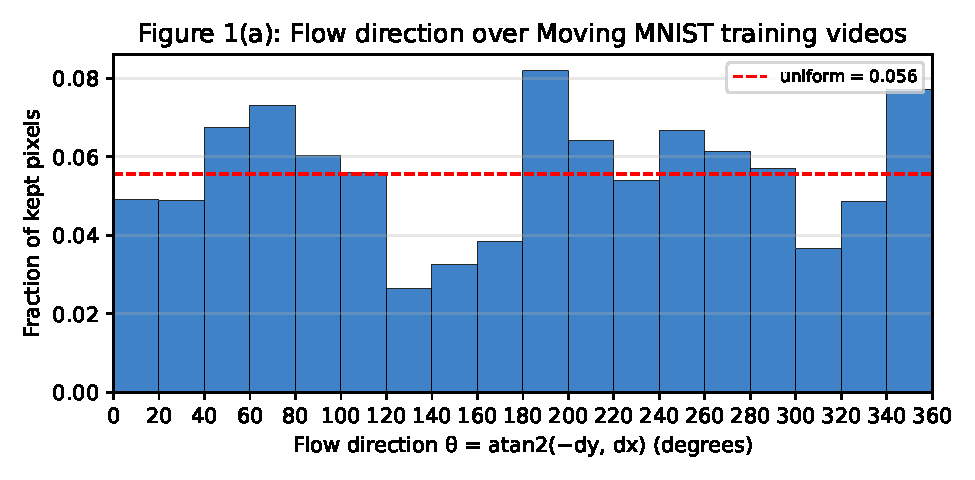
\includegraphics[width=0.49\linewidth]{fig_flow_direction.pdf}
\hfill
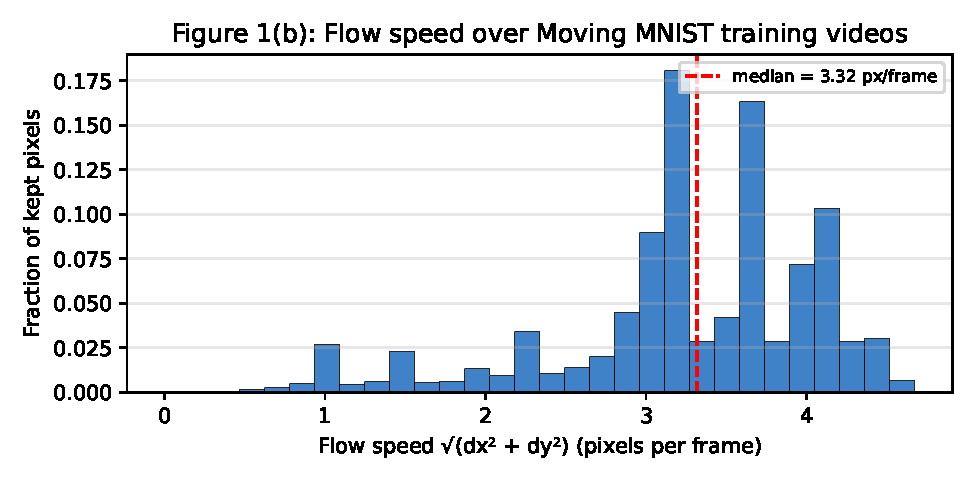
\includegraphics[width=0.49\linewidth]{fig_flow_speed.pdf}
\caption{Optical flow over the first 50 Moving MNIST training videos, pooled over 950 consecutive frame pairs. (a) Histogram of flow direction $\theta = \operatorname{atan2}(-dy, dx)$ in degrees on $[0^\circ, 360^\circ)$ with 18 bins of $20^\circ$; the dashed line marks the uniform level $1/18$. (b) Histogram of flow speed $\sqrt{dx^2 + dy^2}$ in pixels per frame; the dashed line marks the median. 103{,}050 pixels were kept (intensity $> 0.2$ in both frames and flow magnitude $> 0.5$ pixels). Median speed: 3.32 pixels per frame.}
\label{fig:flow}
\end{figure}

\subsection*{Q2.1}

Based on Figure~\ref{fig:flow}(a), mirrored and rotated trajectories would already be familiar in their motion statistics. The histogram is broad and covers every direction: all 18 bins are populated, and the bin fractions lie between about $0.026$ and $0.083$ around the uniform level $1/18 \approx 0.056$. The histogram is not exactly flat because the underlying velocities are discrete and the estimate uses only 50 videos, but no direction is systematically absent. Mirroring reflects the histogram ($\theta \mapsto 180^\circ-\theta$) and rotation shifts it by $90^\circ$; the data-generation process is square-symmetric, so these transformations map the training motion distribution onto itself. What changes is the digit appearance.

From Figure~\ref{fig:flow}(b), a typical digit moves at 3.32 pixels per frame (median over 103{,}050 kept pixels across 950 frame pairs). Running at $2\times$ corresponds to roughly twice that speed in pixels per frame (about 6.64), and $3\times$ to roughly three times (about 9.96). Optical flow is unreliable where the two digits overlap, but overlaps are brief and localised, so they cannot bias the pooled histograms enough to change this conclusion.

\subsection*{Q2.2}

For each transformation:

\begin{itemize}
  \item {Mirror $M$:} changes the {digit appearance} only. The motion statistics (speeds, bounce behaviour, direction distribution) are unchanged, just reflected.
  \item {Rotation $R$:} changes the {digit appearance} only. Motion statistics are unchanged, just rotated.
  \item {Speed-up ($k\times$):} changes the {motion statistics} only (digits move further between frames). Digit appearance is unchanged.
\end{itemize}

This makes the three transformations useful as a controlled experiment because each one isolates a single factor. Mirror and rotation perturb appearance while leaving motion statistics intact, so any failure under them must come from the model tying its motion rule to what the digits look like. Speed-up perturbs motion statistics while leaving appearance intact, so any failure under it must come from the model not having seen or not being able to reach that kind of motion. Comparing the three tells us whether the model's errors are driven by appearance, by unfamiliar motion, or by architectural reach.

\vspace{10pt}
\hrule
\vspace{4pt}

\section*{ConvLSTM Baseline}

\subsection*{Architecture}

Each input frame undergoes
\texttt{pixel\_unshuffle(4)}, folding each $4\times4$ pixel patch into channels: a $1\times64\times64$ frame becomes
$16\times16\times16$. Two ConvLSTM layers follow, each with 64 hidden channels and $3\times3$ kernels (stride 1, zero
padding 1). Layer 1 takes the folded frame; layer 2 takes layer 1's new hidden state. Hidden and cell states start at
zero for every video. A $1\times1$ convolution maps layer 2's hidden state from 64 to 16 channels, then
\texttt{pixel\_shuffle(4)} and a sigmoid give back a $1\times64\times64$ frame.

Each ConvLSTM layer $\ell\in\{1,2\}$, with input $u_\tau$, computes
\begin{align*}
[\,i,\ f,\ o,\ g\,] &= \operatorname{Conv}_{3\times3}\big[\,u_\tau,\ h^{(\ell)}_{\tau-1}\,\big],\\
c^{(\ell)}_\tau &= \sigma(f)\odot c^{(\ell)}_{\tau-1} + \sigma(i)\odot\tanh(g),\\
h^{(\ell)}_\tau &= \sigma(o)\odot\tanh(c^{(\ell)}_\tau),
\end{align*}
where $[\cdot,\cdot]$ is channel concatenation and one convolution produces all four gates. For layer 1,
$u^{(1)}_\tau$ is the folded frame; for layer 2, $u^{(2)}_\tau = h^{(1)}_\tau$. Each layer has its own weights. All
convolutions use a learnable bias and PyTorch's default initialisation. No normalisation, dropout, or residual
connections are added. Model A has exactly 480{,}784 trainable parameters.

\paragraph{Rollout.} The network runs for 9 steps. For $\tau=1,\dots,5$, the input $u_\tau$ is the $\tau$-th input frame;
for $\tau=6,\dots,9$, it is the network's own previous prediction $\hat{x}_\tau$. The outputs of steps 5--9 form
$\hat{Y}=(\hat{x}_6,\dots,\hat{x}_{10})$; the outputs of steps 1--4 are thrown away. No teacher forcing is used: true
future frames are never fed to the network, and gradients flow through the fed-back predictions.

\subsection*{Training and evaluation}

Model A is trained with Adam (learning rate $10^{-3}$, no schedule), batch size 32, for 30 epochs, keeping the final-epoch
weights. One epoch is one pass over the 8{,}000 training videos in shuffled order, with one randomly sampled window per
video ($t\in\{1,\dots,11\}$ at normal speed). The loss is squared error between prediction and target, averaged over the
pixels and the available target frames of each video, then averaged over the videos in the batch. Every model is trained
with seeds 0 and 1; each entry is reported as mean(seed 0, seed 1). The model was trained on an NVIDIA GeForce RTX 5060 Ti GPU (16 GB memory).

\subsection*{Q2.3: Reach of model A}

Model A's reach (the largest distance, in original pixels, that information can travel through the network in one time
step) is 8 pixels. The reasoning:

\begin{enumerate}
  \item \texttt{pixel\_unshuffle(4)} maps each $4\times4$ patch to one cell of the $16\times16$ folded grid. One cell
        corresponds to 4 original pixels (centre-to-centre); the patch width itself is not added.
  \item A $3\times3$ spatial convolution on the folded grid lets information move from a cell to any of its 8 neighbours,
        i.e. by one cell = 4 original pixels in each direction. The $1\times1$ output convolution,
        \texttt{pixel\_unshuffle} and \texttt{pixel\_shuffle} do not move information.
  \item Within one time step $\tau$, consider all paths through the spatial convolutions from the new input
        $u_\tau$ or from the previous states $h^{(1)}_{\tau-1}$, $h^{(2)}_{\tau-1}$ to the prediction $\hat{x}_{\tau+1}$:
        \begin{itemize}
          \item $u_\tau \to$ ConvLSTM layer 1 ($3\times3$ conv) $\to$ ConvLSTM layer 2 ($3\times3$ conv): $+4+4 = 8$ pixels
          \item $h^{(1)}_{\tau-1} \to$ ConvLSTM layer 1 ($3\times3$ conv) $\to$ ConvLSTM layer 2 ($3\times3$ conv): $+4+4 = 8$ pixels
          \item $h^{(2)}_{\tau-1} \to$ ConvLSTM layer 2 ($3\times3$ conv): $+4$ pixels
        \end{itemize}
        The longest path determines the reach.
  \item Total: 8 original pixels per time step.
\end{enumerate}


\subsection*{Model A performance}

\begin{table}[htbp]
\centering
\footnotesize
\begin{tabular}{@{}lccccccc@{}}
  \toprule
 & MSE$_1$ & MSE$_2$ & MSE$_3$ & MSE$_4$ & MSE$_5$ & $E^{(5)}$ & Params \\
 \midrule
\multirow{2}{*}{Model A} & 0.0166 & 0.0203 & 0.0227 & 0.0246 & 0.0264 & 0.0221 & 480784 \\
 & \scriptsize(0.0170, 0.0161) & \scriptsize(0.0209, 0.0197) & \scriptsize(0.0234, 0.0220) & \scriptsize(0.0253, 0.0239) & \scriptsize(0.0270, 0.0257) & \scriptsize(0.0227, 0.0215) & \\
Blank & 0.0426 & 0.0426 & 0.0426 & 0.0426 & 0.0426 & 0.0426 & 0 \\
Copy-last & 0.0492 & 0.0604 & 0.0669 & 0.0708 & 0.0732 & 0.0641 & 0 \\
\bottomrule
\end{tabular}
\caption{Per-horizon MSE and $E^{(5)}$ on the 1,000 test videos for model A and the
two untrained reference predictors ($1\times$, $t=1$). Model A entries are
mean (seed 0, seed 1); parameters are trainable parameter counts.}
\label{tab:model_a}
\end{table}

On the RTX 5060 Ti, training took 4.46\,s per epoch (mean over all 30 epochs;
both seeds). Inference on all 1{,}000 test videos at batch size 32 took
0.313\,s for seed 0 and 0.318\,s for seed 1 under \texttt{model.eval()} and
\texttt{torch.no\_grad()}, starting after each batch was on the device.

\begin{figure}[htbp]
  \centering
  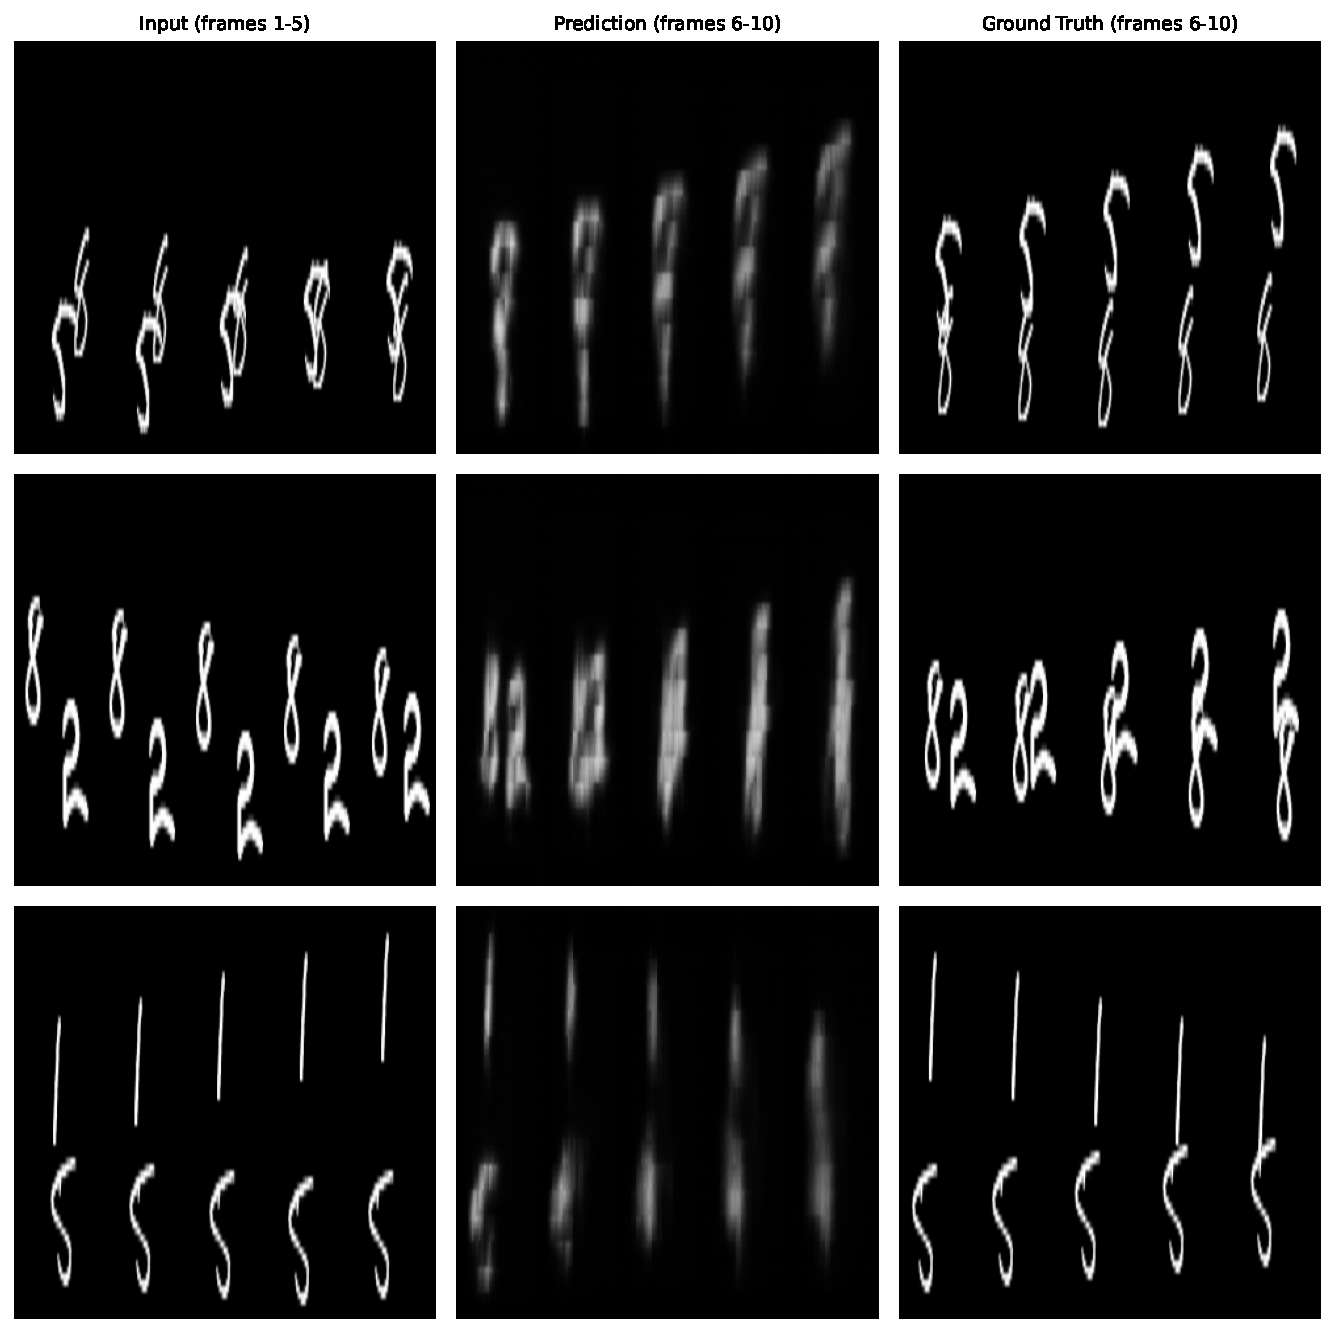
\includegraphics[width=0.9\linewidth]{fig_model_a_predictions.pdf}
  \caption{Input, prediction and ground truth for three test videos from model A (seed 0), including one video with
  overlapping digits (video index 9001 in panel 2).}
  \label{fig:model_a}
\end{figure}

\subsection*{Q2.4: Comparison and error growth}

Model A performs well relative to both baselines, and its error grows smoothly with the
prediction horizon.

From Table~\ref{tab:model_a}, model A's mean per-horizon MSE rises from 0.0166 at horizon 1 to 0.0264 at
horizon 5, while the baseline errors are much larger and flatter. The untrained blank
baseline sits at $E^{(5)}=0.0426$, and the copy-last baseline at $E^{(5)}=0.0641$; model A
achieves $E^{(5)}=0.0221$ on average over the two seeds, roughly half the error of Blank
and about a third of the error of Copy-last.

The per-horizon MSE goes up steadily with the horizon, which is what I expected: each predicted
frame depends on the previous predictions, so errors can build up over the five frames. The gap
to the baselines shows that the ConvLSTM is learning something useful, rather than just
predicting a constant or copying the last frame.


This also fits the reach estimate in Q2.3. At horizon 5 the prediction has been built through five
steps, and each step can only move information by at most 8 pixels, so the error has more time to
build up. The fact that the error is still small (roughly 0.02) at horizon 5, compared with
0.04-0.07 for the baselines, suggests that two stacked $3\times3$ convolutions (reach 8 pixels) are
enough to track a digit at normal speed, which matches the $1\times$ prediction in Q2.5.



In the overlapping test video, model A's prediction gets worse while the digits cross. The two
blobs merge into one blob, and the model does not separate them again in the displayed forecast
window. I think this is because the model is trained with squared error. When the digits overlap,
it cannot tell which digit will come out on which side, so it predicts something like the average
of the possible futures. The result is a blur rather than a clear prediction.

\subsection*{Q2.5: Predictions before running experiments}

Before running any experiment in Testing the Baseline, my predictions are:

\begin{itemize}
  \item \textbf{Mirror:} I expect Model A to fail. It has only seen upright digits, and a mirrored
        digit looks different. I think the filters may have learned the shape of the digits as well
        as their motion, so a flipped digit may not match what they expect.
  \item \textbf{Rotation:} I expect Model A to fail too. Rotation changes the digit shape even more
        than mirroring, and the model has not seen rotated digits in training.
  \item \textbf{Speed:} The reach is 8 pixels per step, and the normal speed is about 3.32
        pixels/frame (Figure~\ref{fig:flow}). At $1\times$ the digit moves less than the reach, so
        the model should be fine. At $2\times$ it moves about 6.64 pixels/frame, which is still
        below 8 but close, so it might start to fail. At $3\times$ it moves about 9.96 pixels/frame,
        which is more than the reach, so the model cannot connect the old and new position in one
        step and should break down.
\end{itemize}

\vspace{10pt}
\hrule
\vspace{4pt}

\section*{Testing the Baseline}

\subsection*{Mirror and rotation}

I ran the handout's two measurements on all 1,000 test videos at $1\times$ with $t=1$, using the
two trained seeds on the same GPU. For $T \in \{M, R\}$ I give the transformed input $T(X)$ to the
model, and I also transform the model's prediction of the original scene; the consistency
measurement is
$\;C_T = \operatorname{MSE}\!\big(f(T(X)),\, T(f(X))\big)\;$ and the correctness measurement is
$\;E_T = \operatorname{MSE}\!\big(f(T(X)),\, T(Y)\big)$, both averaged exactly like $E^{(5)}$.
Figure~\ref{fig:transformations} shows the four worst videos of the seed-0 model,
Table~\ref{tab:transformations} has the full numbers, and Figure~\ref{fig:consistency} shows the
per-video histograms.

\begin{table}[htbp]
  \centering
  \small
  \begin{tabular}{@{}l ccccc@{}}
    \toprule
    Model & $E^{(5)}$ & $C_M$ & $E_M$ & $C_R$ & $E_R$ \\
    \midrule
    \multirow{2}{*}{Model A} & 0.0221 & 0.00190 & 0.0227 & 0.00316 & 0.0239 \\
     & \scriptsize(0.0227, 0.0215) & \scriptsize(0.00187, 0.00193) & \scriptsize(0.0233, 0.0221)
     & \scriptsize(0.00312, 0.00320) & \scriptsize(0.0244, 0.0233) \\
    Blank & 0.0426 & 0 & 0.0426 & 0 & 0.0426 \\
    Copy-last & 0.0641 & 0 & 0.0641 & 0 & 0.0641 \\
    \bottomrule
  \end{tabular}
  \caption{Mirror and rotation on the 1,000 test videos at $1\times$, $t=1$: the consistency gap
  $C$ and the transformed error $E$ at both transformations, next to $E^{(5)}$. Model A entries are
  mean (seed 0, seed 1). Blank and Copy-last are exactly consistent under both transformations, so
  their $C$ columns are 0: their forecasts do not depend on the input content, so a transformed
  scene just gets the transformed version of the same output. Their $E$ columns equal their
  $E^{(5)}$ because under $M$ and $R$ every pixel only moves position, so the squared error against
  the transformed targets is the same as against the originals.}
  \label{tab:transformations}
\end{table}

\begin{figure}[htbp]
  \centering
  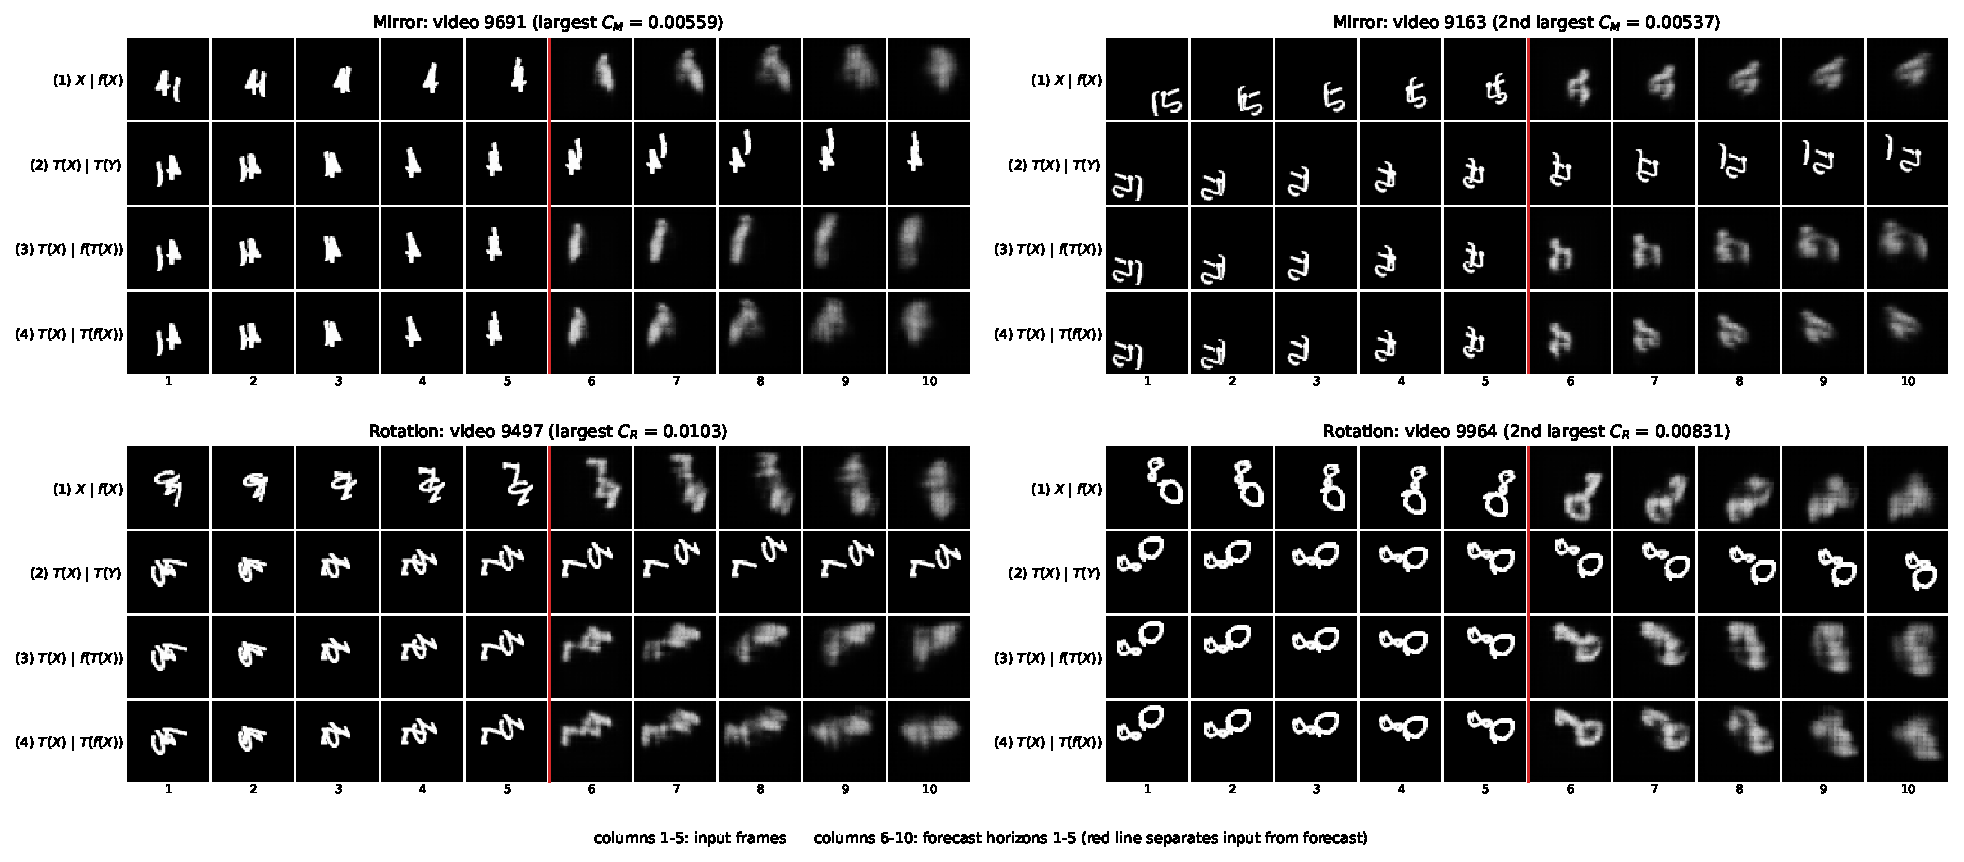
\includegraphics[width=0.98\linewidth]{fig_transformation_panels.pdf}
  \caption{The two test videos with the largest per-video $C_M$ (mirror, videos 9691 and 9163) and
  the two with the largest per-video $C_R$ (rotation, videos 9497 and 9964), for the seed-0 model
  A. Each panel shows four rows of ten frames: columns 1--5 are the input frames and columns 6--10
  are forecast horizons 1--5 (the red line separates input from forecast). Row (1) shows $X$ with
  the normal forecast $f(X)$; row (2) shows $T(X)$ with the true transformed future $T(Y)$; row (3)
  shows $T(X)$ with the forecast from the transformed input $f(T(X))$; row (4) shows $T(X)$ with
  the transformed copy of the normal forecast $T(f(X))$. Rows (3) and (4) agree exactly when the
  transformation carries over to the model.}
  \label{fig:transformations}
\end{figure}

\begin{figure}[htbp]
  \centering
  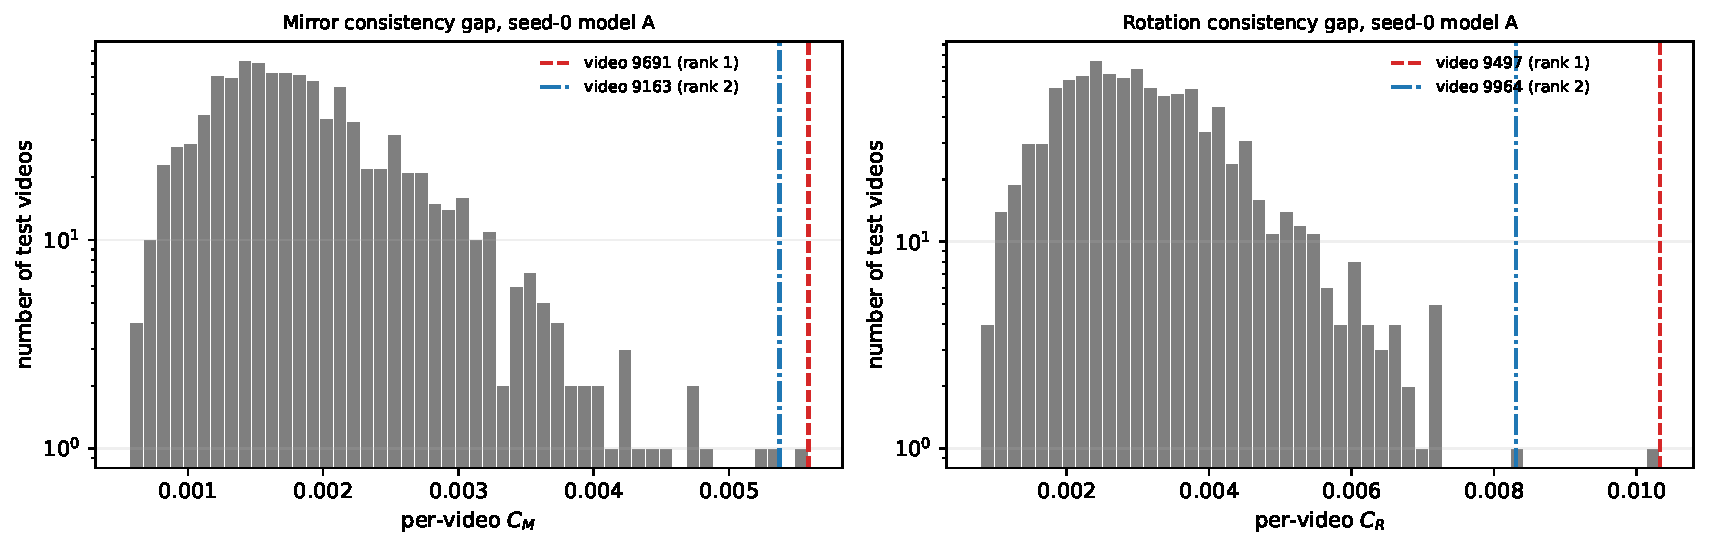
\includegraphics[width=0.9\linewidth]{fig_consistency_histograms.pdf}
  \caption{Per-video consistency on the 1,000 test videos (seed-0 model A): the histogram of
  $C_M$ (left) and $C_R$ (right). The dashed lines mark the videos shown in
  Figure~\ref{fig:transformations}.}
  \label{fig:consistency}
\end{figure}

\subsection*{Q2.6}

Blank and Copy-last are exactly consistent without doing anything that deserves to be called
predicting: Blank always outputs all zeros, and Copy-last just repeats the last input frame. Under
mirror or rotation their outputs move to exactly where their outputs would have been anyway, since
the output does not depend on what the scene contains. So their $C_M$ and $C_R$ are exactly 0.

What this says about reading $C_T$ on its own: a small $C_T$ cannot mean a model is good, because
the most useless predictor wins this test for free. $C_T$ only says that the model treats its own
forecasts the same way as the data under the transformation, and that stays true whether the
forecasts are right or wrong. $E_T$ is the measurement that punishes wrong predictions, so the two
have to go together: $C_T$ tells me whether I can trust the model across a transformation, $E_T$
tells me whether the model has anything worth trusting.

\subsection*{Q2.7}

I take the rotation panel, test video 9497 (largest $C_R = 0.0103$), which is the panel where rows
3 and 4 disagree the most. I looked at the centre of the bright mass of each frame to describe the
drift precisely. In row 2 the true digit moves steadily to the right, about 8 pixels over the five
horizons, keeping roughly the same height. Both forecasts track that drift at first, but both fall
behind the truth. From horizon 3 on the two rows separate: row 3, the forecast from the rotated
input, keeps a nearly straight sideways path a little above the truth, while row 4, the rotated
copy of the normal forecast, slows down further and bends downward, ending by horizon 5 roughly 5
pixels away, down and to the left of row 3. Both rows also lose the digit shape and fade into soft
clouds, so in the last frames neither looks like a digit.

So the model's account of the motion changes under rotation in the sense that the model no longer
produces the rotated version of what it would normally predict: it makes its own call about the
rotated scene, with a different speed and a different bend in the path. This matches the values of
$C_R$ being small overall: the disagreement is a slow sideways split that builds up with the
horizon rather than a wrong direction from the start.

\subsection*{Q2.8}

Rotation is a bit harder for model A than mirroring: $C_R = 0.00316$ against $C_M = 0.00190$
(about $1.7\times$), and $E_R = 0.0239$ against $E_M = 0.0227$, both above the normal
$E^{(5)} = 0.0221$. From my answers to Q2.1 and Q2.2, neither transformation changes the motion
statistics: the direction histogram in Figure~\ref{fig:flow} already covers every direction, so a
mirrored or rotated trajectory is a motion the data produces by itself. If the motion side is unchanged, the
difference between the two tests has to come from the digits' appearance, which is the one thing
$R$ changes more than $M$.

I think the overall message is that the model is only weakly tied to what the digits look like.
Both $E_M$ and $E_R$ stay close to the normal error and far below the baselines, so my prediction
in Q2.5 was wrong: model A does not fail the mirror or the rotation test, it just gets a little
worse. The small extra damage from rotation fits an appearance argument: digits are tall and narrow with
mostly vertical strokes, a mirror keeps them tall with vertical strokes, while a $90^\circ$ rotation
makes them wide with horizontal strokes, which is further from anything the model saw in training.

\subsection*{Faster motion}

Next I rebuilt the test windows at $2\times$ and $3\times$ with $t=1$ (at $3\times$ the video only
has room for two target frames, 16 and 19) and scored model A and Copy-last on all 1,000 test
videos, both seeds, on the same GPU (Table~\ref{tab:speed}); Figure~\ref{fig:speed} shows one test
video played at the three speeds with the seed-0 model.

\begin{table}[htbp]
  \centering
  \small
  \begin{tabular}{@{}l cc cc@{}}
    \toprule
    & \multicolumn{2}{c}{$E^{(2)}$} & \multicolumn{2}{c}{$E^{(5)}$} \\
    Speed & Model A & Copy-last & Model A & Copy-last \\
    \midrule
    \multirow{2}{*}{$1\times$} & 0.0184 & 0.0548 & 0.0221 & 0.0641 \\
     & \scriptsize(0.0190, 0.0179) & & \scriptsize(0.0227, 0.0215) & \\
    \multirow{2}{*}{$2\times$} & 0.0448 & 0.0661 & 0.0497 & 0.0719 \\
     & \scriptsize(0.0443, 0.0454) & & \scriptsize(0.0494, 0.0500) & \\
    \multirow{2}{*}{$3\times$} & 0.0517 & 0.0703 & -- & -- \\
     & \scriptsize(0.0508, 0.0525) & & & \\
    \bottomrule
  \end{tabular}
  \caption{Faster motion on the 1,000 test videos with $t=1$: $E^{(2)}$ over the first two forecast
  horizons and $E^{(5)}$ over all available horizons, for model A (mean of seeds 0 and 1 in the
  small line) and Copy-last. At $3\times$ only two target frames exist (16 and 19), so
  $E^{(5)}$ is not defined there.}
  \label{tab:speed}
\end{table}

\begin{figure}[htbp]
  \centering
  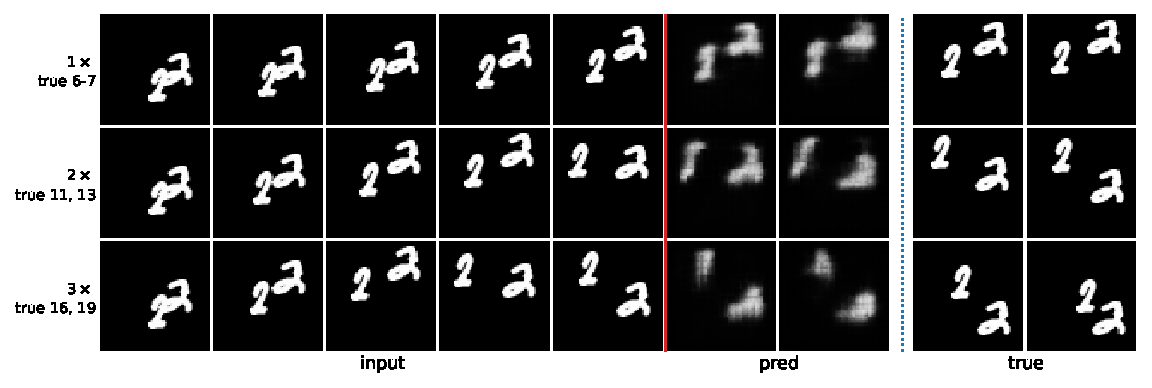
\includegraphics[width=0.86\linewidth]{fig_speed_panels.pdf}
  \caption{Model A (seed 0) on test video 9633 at $1\times$, $2\times$ and $3\times$ with $t=1$:
  five input frames, the first two predicted frames, then the same two true frames (the red line
  separates input from forecast, the dotted line separates prediction from truth). The video was
  picked because its digits do not overlap in any of the displayed true frames (the first three
  input frames do overlap); its per-video
  $E^{(2)}$ is 0.0205 at $1\times$, 0.0642 at $2\times$ and 0.0775 at $3\times$.}
  \label{fig:speed}
\end{figure}

\subsection*{Q2.9}

Model A's predictions fall apart at $2\times$. In Table~\ref{tab:speed}, $E^{(2)}$ jumps from
0.0184 at $1\times$ to 0.0448 at $2\times$ and $E^{(5)}$ goes from 0.0221
to 0.0497, which is even worse than the untrained Blank row (0.0426 in Table 2). At $3\times$ it
stays broken ($E^{(2)} = 0.0517$), though model A still beats Copy-last at every speed.

This agrees with my reach estimate in Q2.3 not fully. The reach said model A must fail at
$3\times$, where a digit moves about 9.96 pixels per step and information can travel at most 8
pixels; at $2\times$ the step is about 6.64 pixels, so the reach alone allowed it to work. What my
estimate missed was that the reach is only a bound on how far information can move between two frames, not
a guarantee that the trained model uses that room. Model A never saw a window where the digits
move about 6.6 pixels or more between the frames it gets, because every training window was
$1\times$, so its filters only ever had to handle steps of about 3.3 pixels. So the breakdown
happens before the bound of Q2.3 is violated, and Table 4 alone cannot split how much is unseen
motion and how much is reach.

This description comes from looking at Figure~\ref{fig:speed} (seed-0 model A, video 9633). The predictions are soft and a little dimmer than the true digits at every speed,
including $1\times$, so blur is not the speed failure. What changes with speed is where the digits
are placed. At $1\times$ the predicted digits sit close to the true ones. At $2\times$ they lag
behind: the predicted masses stay near their positions in the last input frame while the true digits
move on, and the lag grows with the horizon. At $3\times$ the lag is larger, and the smaller digit
becomes fainter and is predicted on the wrong side of its last position. I do not see a duplicated
digit, and no digit disappears completely.

The lag suggests the model applies the motion rule it learned at $1\times$ and does not scale it up
to bigger jumps. The fading suggests that when the input does not fit that rule it hedges between
possible positions, which under squared error gives a faint, soft blob instead of a sharp wrong one.

\subsection*{Q2.10}

From these results alone I cannot tell the two apart. Training never showed $2\times$ or
$3\times$ windows, so the motion is unfamiliar; and the jumps between the given frames at those
speeds (6.64 and 9.96 pixels per step) brush against and pass the 8-pixel reach. Both stories
predict exactly the same thing in Table~\ref{tab:speed}: errors that jump together once the speed
goes up. Nothing in the error numbers tells me which story is the real one.

The experiment that would separate them is to train one more model with the same architecture but
on speed-augmented windows, drawing $k$ from $\{1, 2, 3\}$ for each training window. If the $2\times$ and $3\times$ errors drop to normal levels, the
failure was unfamiliar motion and more data fixes it. If the $3\times$ errors stay bad even though
$3\times$ windows were in the training data, the block would be the reach, and no amount of data carries
the digits faster than the architecture allows.

\subsection*{Q2.11: Prediction before training B--D}

Prediction written before training B--D:

\begin{itemize}
  \item I expect model B to fix the mirror and rotation failures, since its training windows will
        include mirrored and rotated copies of the ordinary windows, so the digit shapes it meets
        at test time are no longer new; I do not expect B to help with speed, since it still trains
        only at $1\times$.
  \item I expect model C to fix the $2\times$ failure and to improve the $3\times$ failure, because
        the jumps that model A never practised will now be in its training data; how much of
        $3\times$ survives depends on whether those jumps are past the 8-pixel reach, where I
        expect extra data to stop helping.
  \item I expect model D, which trains on the same speeds as C but carries information further in
        one step, to be the model that fully fixes $3\times$, and in general I predict the order at
        high speed will be D, then C, then A.
\end{itemize}

\end{document}
